\documentclass[a4paper]{scrreprt}

\usepackage[ngerman]{babel}
\usepackage[utf8]{inputenc}
\usepackage[T1]{fontenc}
\usepackage{ae}
\usepackage[bookmarks, bookmarksnumbered]{hyperref}
\usepackage{tabularx}
\usepackage{graphicx}
\usepackage{csquotes}
\usepackage{verbatim}
\usepackage[nonumberlist, toc, section]{glossaries}
\usepackage[german]{fancyref}

\makeglossaries


% Document
% zu jedem umgesetzten Punkt des Pflichtenhefts Bezug herstellen

\begin{document}

    \tableofcontents
    \chapter{Einleitung}
    \chapter{Architekturdiagramm}

    \chapter{Klassendiagramme}
    \section{API}
    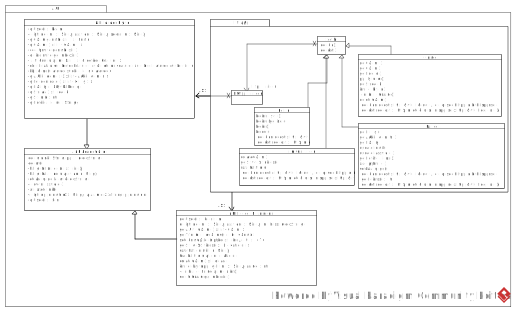
\includegraphics[width=\textwidth]{img/api.png}
    \subsection{APIFacadePlayer}
        Eine APIFacadePlayer ist das Objekt, über welches sämtliche Interaktion mit dem System von den Spielern aus passiert. Eine APIFacadePlayer ist immer mit einem Spieler assziert, falls dieser korrekt angemeldet wurde. Alle Methoden beziehen sich dann auf den angemeldeten Spieler.
    \subsubsection{loginPlayer}
        \begin{itemize}
            \item Beschreibung: Versucht einen Spieler mit email und password anzumelden. Bei Erfolg wird diese Facade mit dem Spieler assoziert.
            \item Parameters: 
                \begin{itemize}
                    \item email: Die Email Adresse mit der eine Anmeldung versucht wird
                    \item password: Das Passwort zu mit dem eine Anmeldung versucht wird
                \end{itemize}
            \item Rückgabewert: Falls die Email-Passwort Kombination einen validen Spieler beschreibt, wird dieser zurückgegeben. Andernfalls wird null zurückgegeben.
        \end{itemize}
    \chapter{Sequenzdiagramme}

    \chapter{Datenhaltung}
        \section{Ordnerstruktur}
        \section{Konfiguration}
        \section{Datenbank}



\end{document}
